\documentclass{article}
\usepackage[utf8]{inputenc}
\usepackage{graphicx}
\usepackage{multirow}
\usepackage{float}
\usepackage{geometry}
\geometry{
	a4paper,
	total={170mm,257mm},
	left=30mm,
	right=30mm,
	top=20mm,
}
\title{Workplan for project A3: Motion Control of Unmanned Aerial Vehicle}

\author{Vilhelm Dinevik \\ Paula Carbó}
\date{\today}
\begin{document}
	\maketitle
	\section{Background}
		Unmanned aerial vehicles, also known as UAVs, are becoming nowadays more and more popular because they are small, cheap to produce, have low operating and maintenance cost, have great maneuverability, can perform steady flight operations and are able to enter high-risk areas without having to compromise human safety. Most applications that involve UAVs have been used in open areas without any obstacles and with a human in control of the UAV. But in recent years people have come up with more modern applications of UAVs that will need this UAVs to fly autonomously in densely populated areas, with a lot of other autonomous UAVs around, e.g. Amazon Prime Air delivery system, AltiGator drones services for inspection and data adquisition, or multi-UAVs used to deploy an aerial communications network. This places high demands on UAVs’ obstacle avoidance capabilities for both moving and static obstacles.
		
		\vspace{1em}
		There is many different manufacturers and a vast amount of different UAV models, all with different motors, weights, sensors and lift-to-weight ratio. To make a standard autonomous flight applicable to all these kinds of UAVs, a simple and easy-to-implement multi-UAV mathematical model, that will still be able to avoid obstacles with as few sensors as possible, is needed.  
		
		\vspace{1em}
		This project aims to study and develop a mathematical model of a quadrotor UAV and the available sensors in it.  From the trajectory and pose tracking a state feedback controller will be designed. In order to facilitate the multi-UAV navigation potential fields or an A* algorithm will be used to make several quads fly to their goals mantaining collision avoidance with respect to other quads and obstacles. To check the validity of the models, a simulated test environment in MatLab filled with a random reasonable amount of static obstacles and autonomous UAVs will be used.
		
		
		
	\section{Work tree}
		\begin{figure}[H]
				\centering
				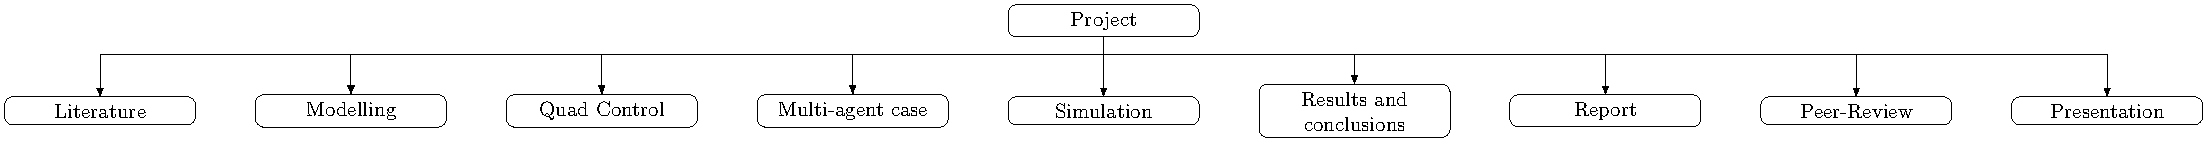
\includegraphics[width=\linewidth]{Workplan_work_tree/basic_work_tree_diagram}
				\caption{Basic work tree}
		\end{figure}
		\begin{figure}[H]
			\centering
			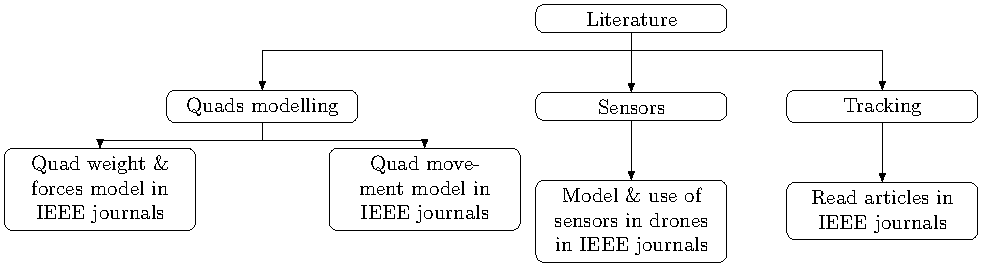
\includegraphics[width=.8\linewidth]{Workplan_work_tree/literature_work_tree_diagram}
			\caption{Expanded work tree for the literature section}
		\end{figure}
		\begin{figure}[H]
			\centering
			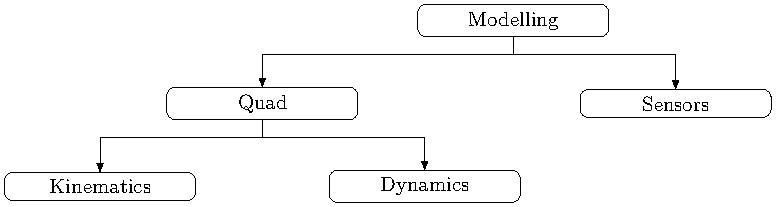
\includegraphics[width=.8\linewidth]{Workplan_work_tree/modelling_work_tree_diagram}
			\caption{Expanded work tree for the modelling section}
		\end{figure}
		\begin{figure}[H]
			\centering
			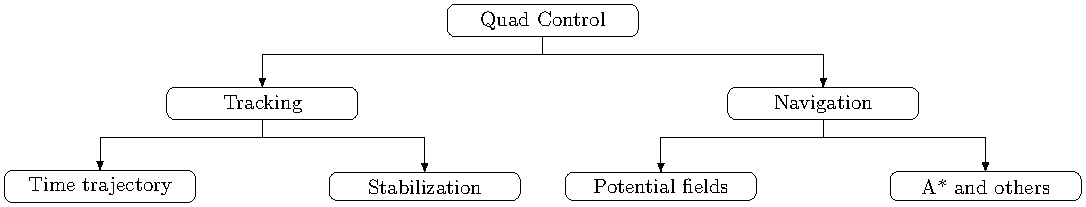
\includegraphics[width=.8\linewidth]{Workplan_work_tree/control_work_tree_diagram}
			\caption{Expanded work tree for the single-quad control section}
		\end{figure}
		\begin{figure}[H]
			\centering
			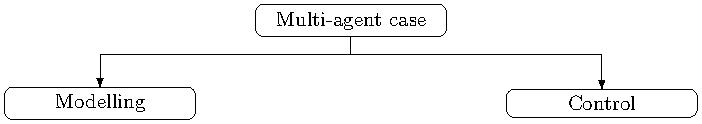
\includegraphics[width=.8\linewidth]{Workplan_work_tree/multiagent_work_tree_diagram}
			\caption{Expanded work tree for the multi-agent case section}
		\end{figure}
		\begin{figure}[H]
			\centering
			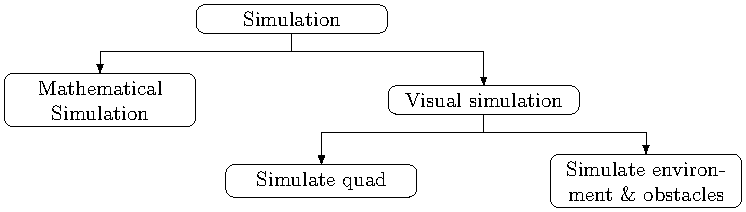
\includegraphics[width=.8\linewidth]{Workplan_work_tree/simulation_work_tree_diagram}
			\caption{Expanded work tree for the simulation section}
		\end{figure}

			
	
	\section{Risks}
		\begin{tabular}{|l|c|c|c|r|}			
			Risks & P & C & R & Counter measure \\
			\hline
			Diseases in the group  & 2 & 2 & 4 & Reactive:rearrange workload 				\\ & & & & Proactive: Nothing \\
			
				
		\end{tabular}		
	\section{Goals}
		
	\section{Time line}
	
\end{document}
